\documentclass[border=4pt]{standalone}
\usepackage{tikz}
\usetikzlibrary{arrows.meta,shapes.geometric}
\begin{document}
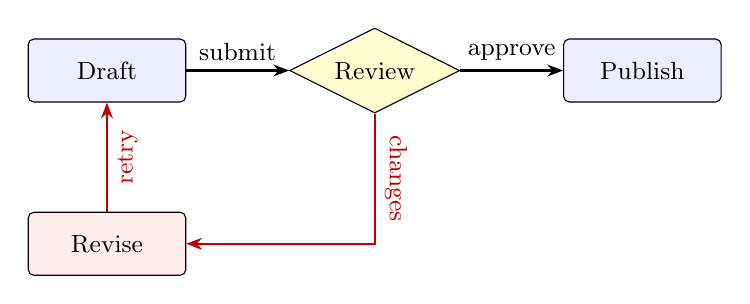
\begin{tikzpicture}[
  auto,
  stage/.style={draw,rounded corners=2pt,minimum width=20mm,minimum height=8mm,fill=blue!7},
  gate/.style={draw,diamond,aspect=2,minimum width=20mm,minimum height=10mm,fill=yellow!18},
  flow/.style={-{Stealth[length=2mm]},thick},
  every node/.append style={font=\small}
]
  \node[stage] (draft) at (0,0) {Draft};
  \node[gate] (review) at (3.4,0) {Review};
  \node[stage] (publish) at (6.8,0) {Publish};
  \node[stage,fill=red!7] (revise) at (0,-2.2) {Revise};

  \draw[flow] (draft) -- node[pos=.5,sloped] {submit} (review);
  \draw[flow] (review) -- node[pos=.5,sloped] {approve} (publish);
  \draw[flow,red!75!black] (review.south) |- node[pos=.25,sloped] {changes} (revise.east);
  \draw[flow,red!75!black] (revise.north) -| node[pos=.75,sloped,swap] {retry} (draft.south);
\end{tikzpicture}
\end{document}
